
\section{Model-Card Integrity Audit}
\label{sec:cards}

The estate's public face is its set of model cards, and the November 14 stamping incident (Section~\ref{sec:incident}) made card integrity a first-class measured property. A full audit of all \textbf{183 model repositories} in the organization (the authenticated denominator; see the instrument caveat in Section~\ref{sec:census}) classified cards by evidence class:
\begin{itemize}
\item \textbf{5} \emph{rich} cards: evidence passport plus at least one MEASURED section (e.g., the Khipu and chaski family flagships);
\item \textbf{59} \emph{receipt-bound} cards: each measured section bound to a named receipt artifact (including all 40 \texttt{-v2-trained} wave-4 repositories);
\item \textbf{7} \emph{passport-no-measure} cards: evidence passport present, no measured section claimed;
\item the \textbf{remaining 112} repositories fall outside the three measured classes (honest-minimal cards, private-by-design worker adapters, and placeholders); their per-card state is recorded in the estate audit receipts.
\end{itemize}

\begin{figure}[htbp]
\centering
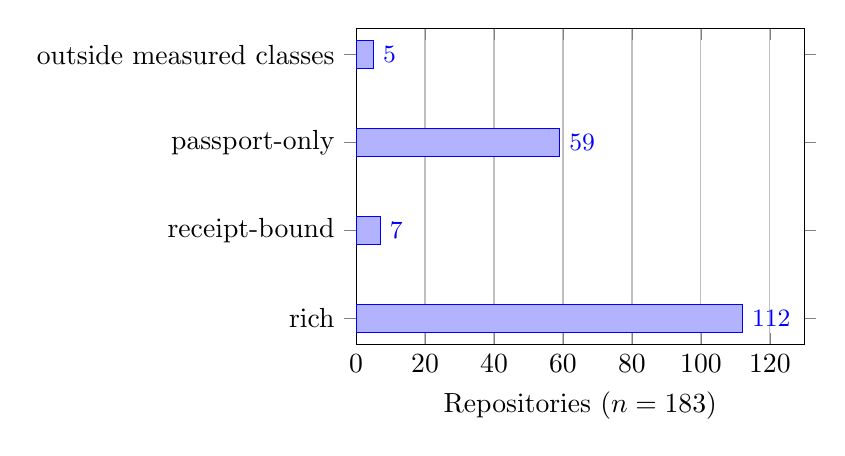
\begin{tikzpicture}
\begin{axis}[
  xbar, width=0.6\textwidth, height=5.6cm,
  symbolic y coords={remainder, passport, receipt-bound, rich},
  ytick=data, xmin=0, xmax=130,
  yticklabels={outside measured classes, passport-only, receipt-bound, rich},
  xlabel={Repositories ($n=183$)},
  nodes near coords, every node near coord/.append style={font=\small},
  xmajorgrids=true,
]
\addplot coordinates {(5,rich) (59,receipt-bound) (7,passport) (112,remainder)};
\end{axis}
\end{tikzpicture}
\caption{Card-evidence classification of the 183 model repositories (November 14--15, 2026 audit). The audit's three measured classes are reported exactly; the remainder is explicitly not smoothed into them.}
\label{fig:cards}
\end{figure}

\paragraph{Re-stamp detection, measured.} A follow-up sweep for stamp residue flagged 43 cards by substring match, and all 43 were verified \textbf{false positives}: the flagged string occurs inside the estate's own honest disclosure cards (which quote the incident signature). The measured result is \textbf{zero re-stamps} across all 183 repositories. Two detection lessons are now doctrine: after convergence, a raw substring is no longer a re-stamp marker (the detector must require the uniform model-index + metrics + QLoRA-table signature instead), and incident disclosures must be distinguishable from incidents.

\paragraph{Identity binding, measured.} The estate binds an identity mark to every card without changing any content claim: after the incident-era restoration, a CAS-based binding pass (45 cards already carried the mark; 138 newly bound via content-addressed upload with SHA-256 old/new logging in \texttt{oro\_bind\_log.jsonl}) produced a verification sweep of \textbf{183 with-mark, 0 without, 0 errors} (Figure~\ref{fig:oro}). The mark is identity-only; the incident ceiling on blanket campaigns stands.

\begin{figure}[htbp]
\centering
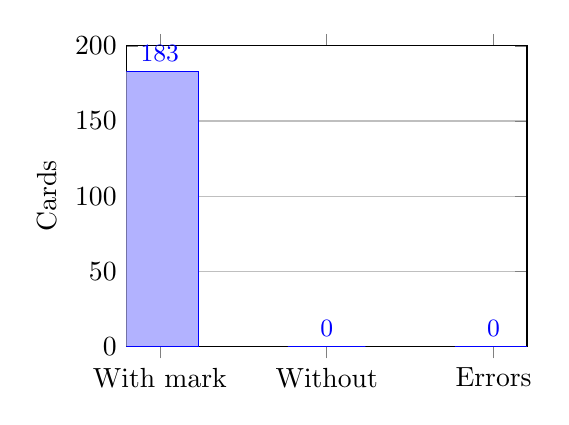
\begin{tikzpicture}
\begin{axis}[
  ybar, bar width=28pt,
  width=0.55\textwidth, height=5.4cm,
  symbolic x coords={With mark, Without, Errors},
  xtick=data, ymin=0, ymax=200,
  ylabel={Cards},
  nodes near coords, every node near coord/.append style={font=\small},
  ymajorgrids=true,
]
\addplot coordinates {(With mark,183) (Without,0) (Errors,0)};
\end{axis}
\end{tikzpicture}
\caption{Identity-bind verification sweep over the 183 model cards (November 2026). A 183/0/0 sweep is the only kind of completeness claim the doctrine permits: measured, not asserted.}
\label{fig:oro}
\end{figure}

\section{Edge Delivery Chain: Operational Case Studies}
\label{sec:edge}

The estate runs its own delivery chain: a Hub-sync pipeline that deploys Spaces, binds sources, attests, live-verifies, and admits the runtime. Its failure modes are as instructive as its successes, and both are receipted.

\subsection{The concurrent-push admit race}
The pipeline's admit stage requires a bracketed readback: the Space's \texttt{runtime.sha} before and after the deploy must bracket to the expected boot identity. On November 14, with roughly forty concurrent operator lanes dispatching deploys, a run failed its \texttt{RUNTIME\_READBACK} stage: the \texttt{runtime.sha} churned three times within minutes (\texttt{76812903}~$\to$~\texttt{80dcd856}~$\to$~\texttt{cf028c03}) as other lanes pushed, breaking the \texttt{before==after} identity bracket. The failure sanitized to \texttt{EXECUTION\_HANDOFF\_UNAVAILABLE}; a duplicate lane run failed identically. The proof that the pipeline itself was healthy came from a quiet-window dispatch: run \texttt{43637549333}, dispatched once the fleet quieted, completed the full admit--parity--re-authorize sequence successfully. The fix was operational, not code: serialize dispatches through a single owner lane. The estate records this as the canonical example of a failure that is a race, not a defect --- and of a diagnosis that distinguishes the two.

\subsection{Live parity and edge fixes}
The live estate is probed continuously; a November 15 probe sweep returned HTTP 200 across the surface (apex, \texttt{mcp-healthz}, atlas, router, \texttt{killinchu}, showcase, the a11oy Space, the org card), with the honest-status endpoint reporting \texttt{git\_sha} \texttt{47a9116d} equal to the repository main HEAD (verified twice). A same-day edge fix eliminated a preflight failure on the monetization route: \texttt{OPTIONS} on the inference host moved from 530/1033 to \textbf{200} with \texttt{Access-Control-Allow-Methods: GET, POST, DELETE, OPTIONS} and \texttt{Allow-Headers: *}, and the apex returned 200 with the edge header \texttt{a11oy-product-edge-v3}. The custom domain \texttt{a-11-oy.com} reports READY at the Hub.

\section{GPU Fleet and Training Receipts}
\label{sec:fleet}

Training runs on a rented GPU fleet under the same receipt discipline. The fleet API census (the provider's container listing) recorded 24 containers across the project during the window; the named training lanes active on November 14 included \texttt{wave4-train}, \texttt{brain-v35-v2}, \texttt{hatun24-train-v2}, and the \texttt{mesh-bench-4090-v2}/\texttt{5090-v2} benchmark lanes, with the crash-looping quartet repatched to running state the same day. Fleet state is re-readable from the provider API with the estate's key; the census times are in the fleet receipts. The fleet census of November 14 recorded \textbf{9 container groups running and 3 allocating} (of a 24-container census across the API), with all five SaladCloud lanes live after a same-day repatch of four crash-looping containers. Fleet receipts are published as they are written: the \texttt{mesh/} namespace of \texttt{frontier-54-runs} grew from a 36-file baseline to \textbf{113 mesh/salad receipt files} in one day (Figure~\ref{fig:fleetreceipts}), and nine Salad worker model repositories are live. The \texttt{wave-logs} dataset carries \textbf{65 genuine training logs} (loss curves from real runs) --- the estate's only source for per-model training claims; models without a log in it are claimed to have none, not to have good ones.

\begin{figure}[htbp]
\centering
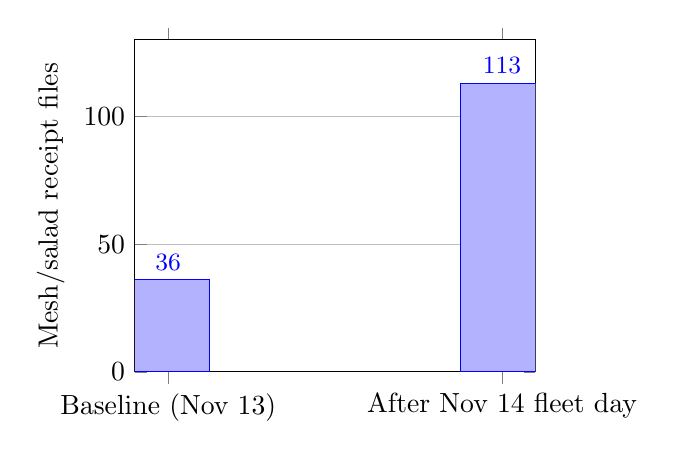
\begin{tikzpicture}
\begin{axis}[
  ybar, bar width=30pt,
  width=0.55\textwidth, height=5.8cm,
  symbolic x coords={Baseline (Nov 13), After Nov 14 fleet day},
  xtick=data, ymin=0, ymax=130,
  ylabel={Mesh/salad receipt files},
  nodes near coords, every node near coord/.append style={font=\small},
  ymajorgrids=true,
]
\addplot coordinates {(Baseline (Nov 13),36) (After Nov 14 fleet day,113)};
\end{axis}
\end{tikzpicture}
\caption{Growth of the fleet receipt namespace across the November 14 training day. Every bar increment is a worker-run receipt, not an estimate.}
\label{fig:fleetreceipts}
\end{figure}

\section{Change Management Receipts}
\label{sec:change}

Every merge to a protected main is itself a receipted event. On November 14 alone, the evening merge ledger records eleven merges across five repositories: a11oy \#3415, \#3383, \#3385, \#3419, \#3340, \#3386 (landing main at \texttt{c7f94397}, 19:46:27Z), \#3388, and \#3421 (squash \texttt{0bb58a5e}, 20:34:25Z, checks 124 pass / 1 non-required parity fail), safe-stack \#41, platform \#1051, and szl-org-health \#334; the next morning a11oy \#3430 (a contract repair stripping 74 stray keys and restoring four Spaces) merged as \texttt{b7397d3}, G-signed, with 34/34 local unit tests green pre-push. Standing doctrine: \textbf{never force-push a protected main}; all changes flow through the merge queue, and a non-required red check does not silently block or bypass --- it is recorded. One tooling lesson is codified: the conventional-commit lint accepts only \texttt{feat|fix|docs|style|refactor|perf|test|build|ci|chore|revert} types, so cross-system sync PRs are titled \texttt{chore} rather than invented types.

\begin{table}[htbp]
\centering
\small
\begin{tabular}{llr}
\toprule
\textbf{Repository} & \textbf{Merges (Nov 14)} & \textbf{Recorded state} \\
\midrule
\texttt{a11oy} & \#3415, \#3383, \#3385, \#3419, \#3340, \#3386, \#3388, \#3421 & main $\to$ \texttt{c7f94397} \\
\texttt{szl-safe-stack} & \#41 & green \\
\texttt{platform} & \#1051 & green \\
\texttt{szl-org-health} & \#334 & green \\
\bottomrule
\end{tabular}
\caption{The November 14 evening merge ledger (a representative window of the change-management receipts; the full ledger is the repositories' own histories, which is the point: the receipt and the artifact are the same object).}
\label{tab:merges}
\end{table}

\section{Publication Track: The Endorsement-Gated Flow, Measured}
\label{sec:pubtrack}

The estate's papers vertical publishes under the target platform's own gate rather than around it, and the flow itself became a measured object during the census. The two companion papers (25 and 26 pages, primary classification \texttt{cs.LO}) are compiled, staged, and bound to a submission record whose start-step form was completed through the platform's real interface: authorship attested, archive and subject class set, license chosen (CC BY 4.0), and the submission agreement accepted. The platform then imposed its first-submission endorsement gate.

\paragraph{Endorser qualification, measured under the platform's own instrument.} Before sending any ask, the estate measured qualification with the platform's own per-user qualification pages: of \textbf{seven} candidate endorsers examined, \textbf{three} were qualified to endorse \texttt{cs.LO} (the papers' primary class), and \textbf{four} were not (qualification in other archives or no qualifying record). The asks were then sent only to qualified addresses, and each ask carried the full proof analytics: the proof repository and its frozen snapshot, the locked-eight registry, the declaration baseline, the receipt dataset addresses, the admission-gate series, and the Track A campaign results. The platform's six-character endorsement code is bound to the submission record; the papers publish when the gate clears, and not before. The estate records the doctrine point explicitly: \textbf{no pressure on endorsers, no mass-asking}, and the qualification census prevented exactly the embarrassment of asking an unqualified party.

\paragraph{A disclosed mismatch, not smoothed.} The submitting account's affiliation of record reads \emph{Independent Researcher}, while the papers carry \emph{SZL Holdings, Inc.} as the author affiliation. The mismatch is visible to any reader and is recorded here rather than silently harmonized: harmonizing the account affiliation is an owner action on the platform, taken (or not) as a deliberate decision, never as an edit-in-passing.

\section{Security Disclosures}
\label{sec:security}

A receipt-first estate must receipt its own security posture, including the unflattering parts. During the census window, transcript forensics (the same method that identified the stamping writer of Section~\ref{sec:incident}) established that a fleet-provider API key and a Hugging Face worker token were present in plaintext across operator transcripts. The exposure class is recorded honestly: the worker token held organization write access and was \emph{stamp-capable} --- the same capability class as the incident writer.

The estate's recorded response is two-part. Immediately: exposure containment by procedure (the plaintext transcripts are operator-side artifacts, and the detection method is now part of the audit kit). Structurally: the standing recommendation is a scoped replacement token for workers (candidate-repository write only), distinct from personal and main tokens. The owner decision at census time was \textbf{no immediate rotation}, recorded with its risk acceptance rather than presented as a completed remediation. No credential value appears in this paper or in any receipt; the disclosure is of the exposure \emph{class} and its disposition, which is the part a reader can audit.
